\chapter{IMPLEMENTATION}

\section{Implementation process}

The implementation involves multiple steps: conceptual design of the DSL, creating the grammar, the lexer and parser, the testing functionality, and testing the DSL itself. Finally, it will be connected all together to work as a fully-fledged Domain Specific Language.

Conceptual design involves specifying the domain of the DSL, what problems it solves, defining use cases, how it will work, what it should and should not do.

Grammar is based on the syntax defined on the previous step. It involves knowing what types and functionality the language will contain.

There are different tools to implement a Domain Specific Language. ANTLR (ANother Tool for Language Recognition) is one of them. It gives a powerful parser that can be used for reading, processing, executing, or translating structured text or binary files. It works by defining a grammar. Then ANTLR creates a parser along with a parse tree. The parser can be used to parse code in the DSL and to apply different actions, which are written in the target language. The actions will do the unit testing behind the scenes for the scenarios specified for testing by the DSL.

There is another tool textX, inspired by a language workbench for building DSLs in java: Xtext. It is a meta-language for textual DSLs in Python. It is similar to ANTLR. Given a grammar description it builds a meta-model as Python classes and a parser for the language. The parser will automatically build a graph of Python objects corresponding to the meta-model. Other features include:
\begin{itemize}
    \item Automatic Abstract Syntax Tree construction
    \item Automatic linking, which allows to have references to other objects in the language and the textual representation of the reference will be resolved automatically
    \item Automatic parent-child relationships imposed by the grammar
    \item Parser configuration, to allow control of the whitespace characters, cases, keyword handling
    \item Model/object post-processing: validation, additional changes etc.
    \item Grammar modularization: grammar can be split across multiple files and imported when necessary
    \item Scope providers
    \item Multiple meta-models support
    \item Meta-model or model visualization with the GraphViz package
\end{itemize}

Xtext, that textX is based on, uses as a default a Concrete Syntax (CS) first approach. From a concrete syntax definition, an abstract syntax (AS) is derived. This is convenient. Though, the resulting AS may not be as clean as if it was derived manually.  The tool supports AS first approach too.

It was used a parser, this means that the abstract syntax tree (AST) is constructed from the CS of a program text. It instantiates and populates the AS, based on the information in the program.

\section{Working in ANTLR}
ANother Tool for Language Recognition (ANTLR) is a powerful tool for creating parsers, interpreters, compilers, and other language processing tools.

The grammar definition developed specifies the syntax for a testing domain-specific language (DSL). The grammar defines several rules that describe how the testing DSL should be structured.

\begin{verbatim}
grammar grammar_antlr;

suite: 'Suite' ID (test | order)*;
test: 'Test' ID flag* 'When' parameter+ result;
flag: '-' ('skip' | 'Skip' | 'Repeat' INT 'times');
parameter: ID '=' datatype | emptyParameters;
result: 'Then' ('result' 'should' 'be')? (datatype | emptyResult);
emptyParameters: 'no' 'parameters' | 'None' | 'none' | 'void' | 'Void';
emptyResult: 'empty' | 'Empty' | 'void' | 'Void' | 'none' | 'None';
order: 'Execution' 'order' ':' ID (',' ID)*;

datatype: STRING | INT | FLOAT | NUMBER | BOOL;
ID: [a-zA-Z_] [a-zA-Z0-9_]*;
STRING: '"' ~'"'* '"';
NUMBER: INT | FLOAT;
INT: [0-9]+;
FLOAT: [0-9]* '.' [0-9]+;
BOOL: 'true' | 'false';

WS: [ \t\r\n]+ -> skip;
\end{verbatim}

The first rule is "suite", which specifies that a suite consists of the word "Suite" followed by an identifier (ID) and zero or more tests or orders.

The second rule is "test", which specifies that a test consists of the word "Test" followed by an identifier, zero or more flags, the word "When", one or more parameters, and the word "Then" followed by an expected result.

The "flag" rule defines the optional flags that can be associated with a test, such as "skip" or "repeat".

The "parameter" rule defines the parameters that can be passed to a test.

The "result" rule defines the expected result of a test.

The "emptyParameters" and "emptyResult" rules define possible values for empty parameters and empty results, respectively.

The "order" rule specifies the execution order for the tests.

Finally, the "datatype" rule defines the possible data types for parameters and results, including strings, integers, floats, and booleans.

The grammar also defines the "WS" rule, which specifies that whitespace characters should be ignored.


\section{Converting tests into JSON}

Converting the tests generated from the grammar into JSON can provide compatibility with other programming languages and tools that can read and parse JSON. This allows the tests to be used in different contexts and environments, such as in continuous integration and deployment pipelines, where different programming languages and tools may be used.

JSON is a widely used data interchange format that is lightweight, easy to read and write, and can be easily consumed by a wide range of programming languages and tools. By converting the tests into JSON, they can be easily shared and used across different systems and platforms. Additionally, JSON is human-readable and can be easily understood by developers, which can make it easier to debug and troubleshoot issues in the tests.

In figure 4 there is a representation of a test implementation of the domain specific language for unit testing that was created.

{ \centering 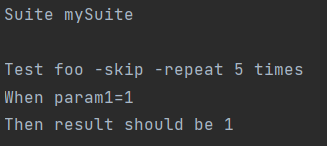
\includegraphics[width=\textwidth , height=6cm]{images/test1.png} }
\begin{center} Figure 4: Test example \end{center}

As noticed, in figure 5, the test was generated as a JSON in a external file.The advantage of converting the tests generated from the grammar into JSON is that it provides a standardized format that can be easily parsed and used to work with different programming languages.

{ \centering 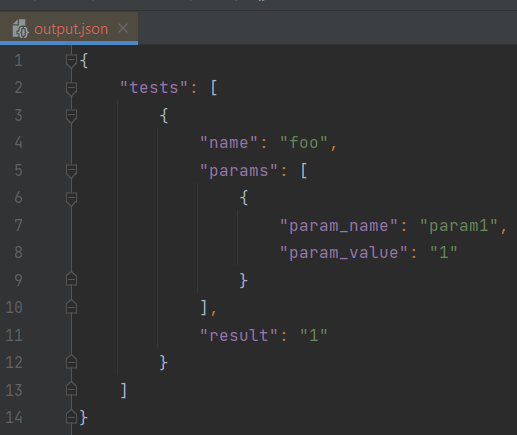
\includegraphics[width=\textwidth, height=12cm]{images/output.png} }
\begin{center} Figure 5: JSON output file  \end{center}

